\subsection{Introduction}


bla


\subsection{Methods}
In this replication, we focus on the rate models proposed in the original article.
The firing rate model was an extensions of the traditional Wilson-Cowan model \supercite{Wilson1972} and represented
an iso-frequency unit of the auditory cortex. This iso-frequency unit consisted of one excitatory and two inhibitory populations.
Building on this unit a more complex three-unit rate models was developed, to investigate stimulus-specific adaptation, forward suppression,
tunig-curve adaptation and feedforward functional connectivity. 

\paragraph{Iso-Frequency Unit Model}

\paragraph{Three-Unit Model}


\subsection{Reproduction of experiments}


\begin{figure}
 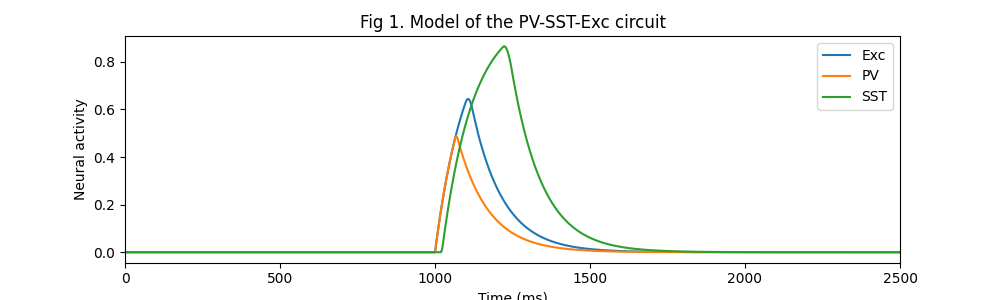
\includegraphics[width=\textwidth]{Figures/Fig1}
 \caption{ReFig1}
\end{figure}

\begin{figure}
 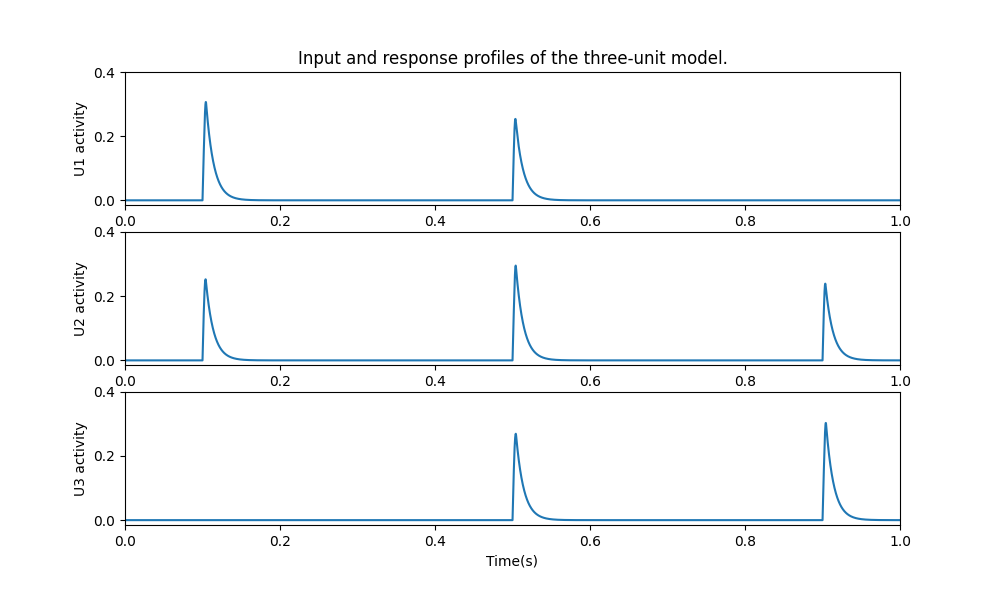
\includegraphics[width=\textwidth]{Figures/Fig2}
 \caption{ReFig2}
\end{figure}

\begin{figure}
 
 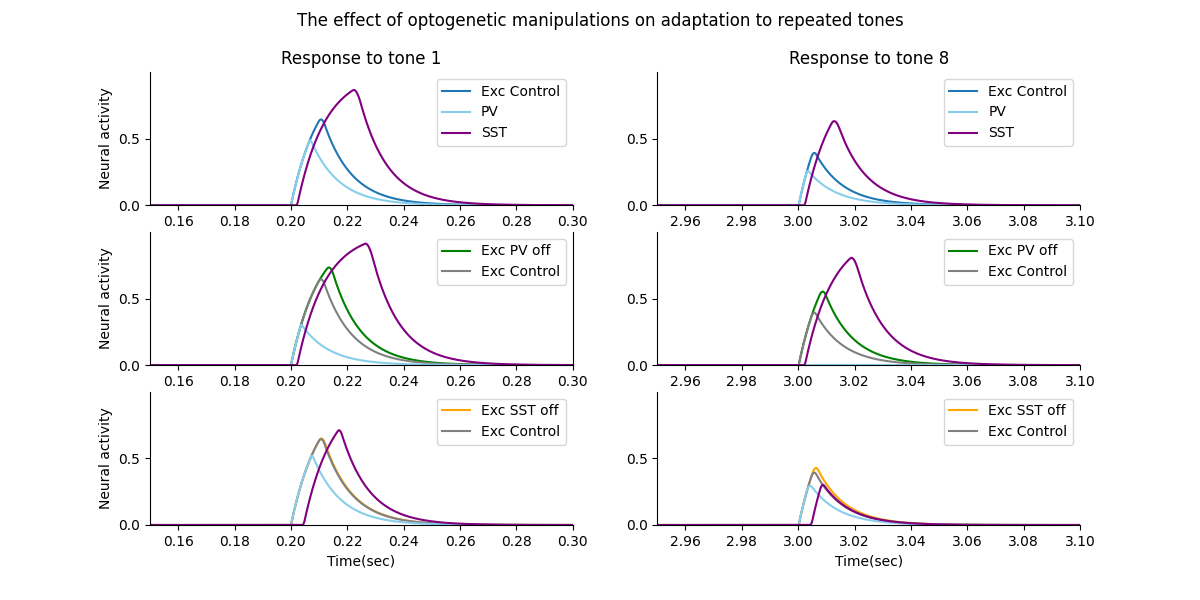
\includegraphics[width=\textwidth]{Figures/Fig3B}
 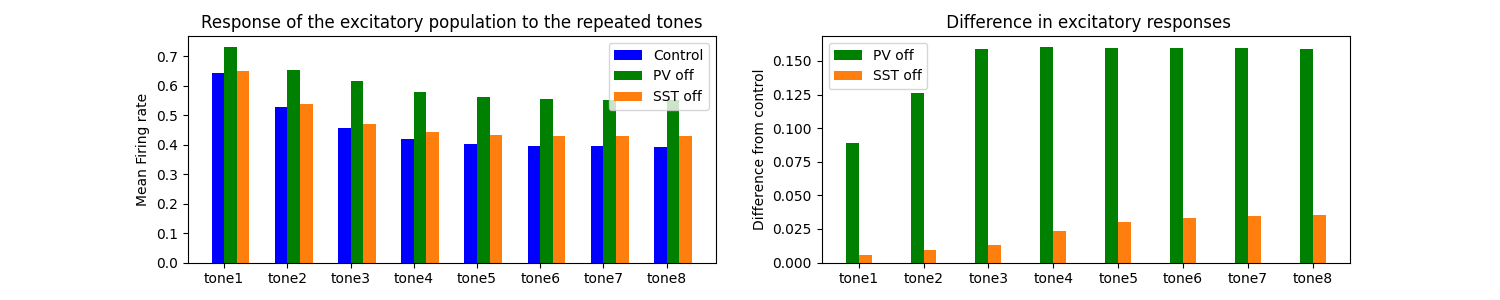
\includegraphics[width=\textwidth]{Figures/Fig3C}
 \caption{ReFig3}
\end{figure}

\begin{figure}
 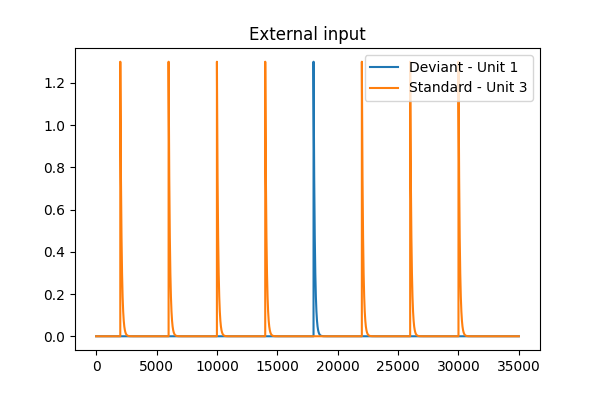
\includegraphics[width=\textwidth]{Figures/Fig4A}
 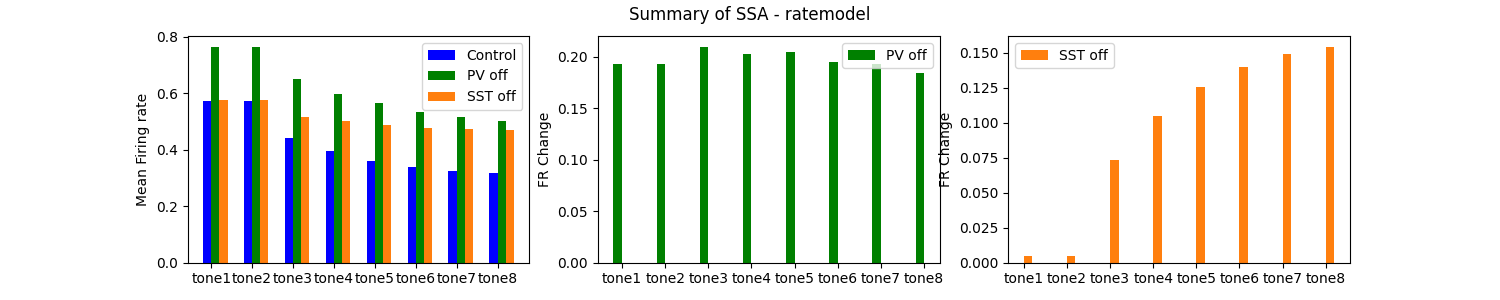
\includegraphics[width=\textwidth]{Figures/Fig4BDE}
 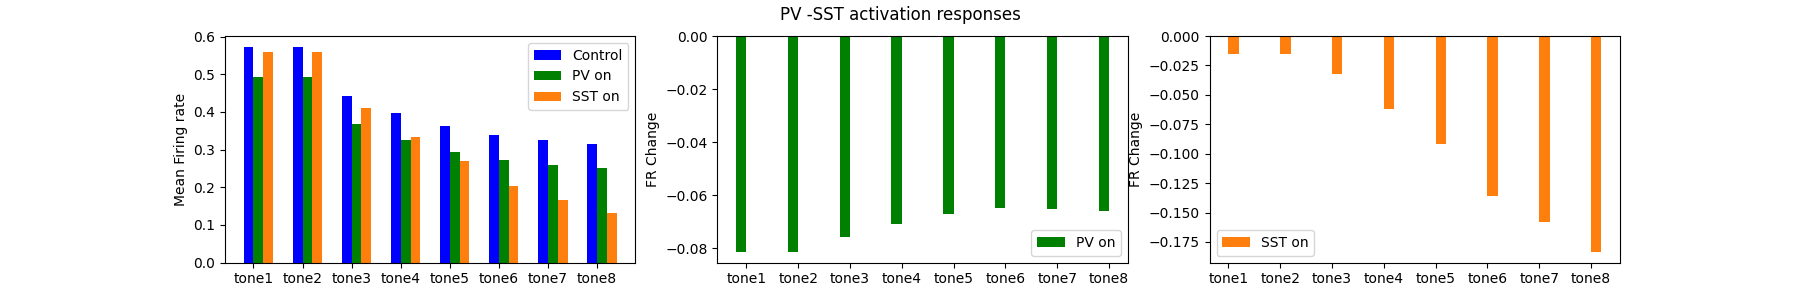
\includegraphics[width=\textwidth]{Figures/Fig4F}
 \caption{ReFig4}
\end{figure}

\begin{figure}
 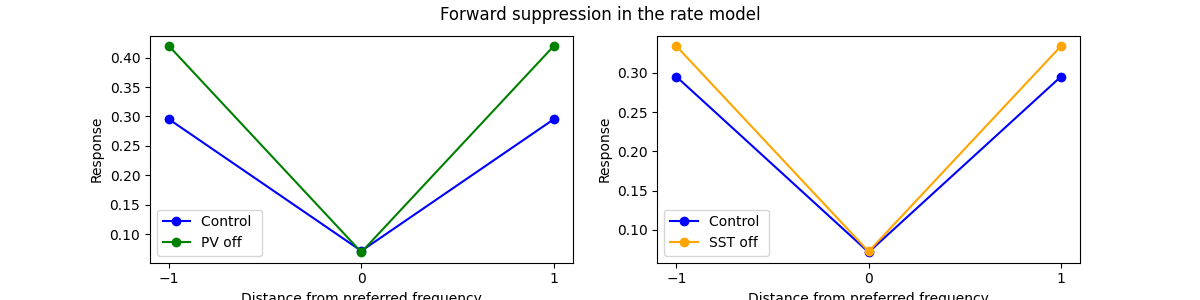
\includegraphics[width=\textwidth]{Figures/Fig6BC}
 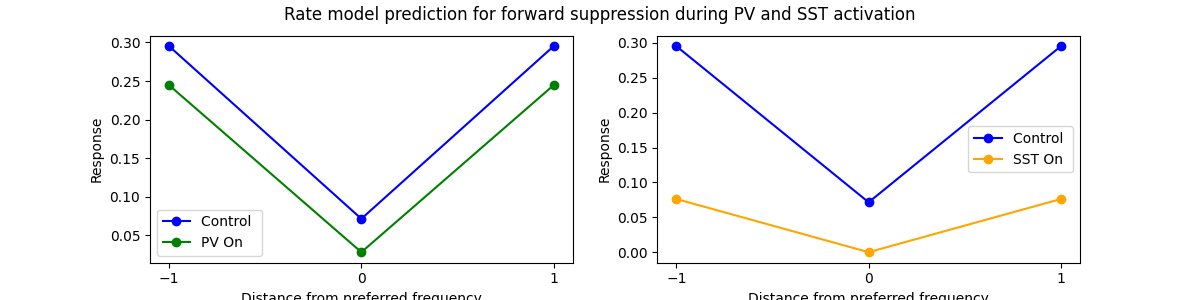
\includegraphics[width=\textwidth]{Figures/Fig6DE}
 \caption{ReFig6}
\end{figure}

\begin{figure}
 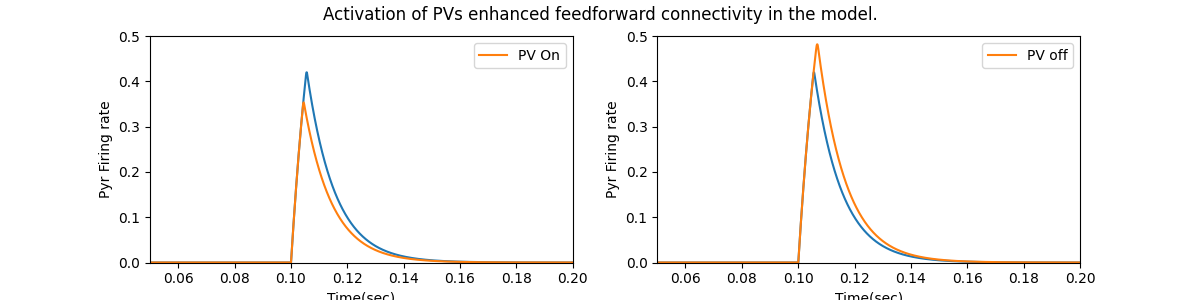
\includegraphics[width=\textwidth]{Figures/Fig8BD}
 \caption{ReFig8}
\end{figure}

\begin{figure}
 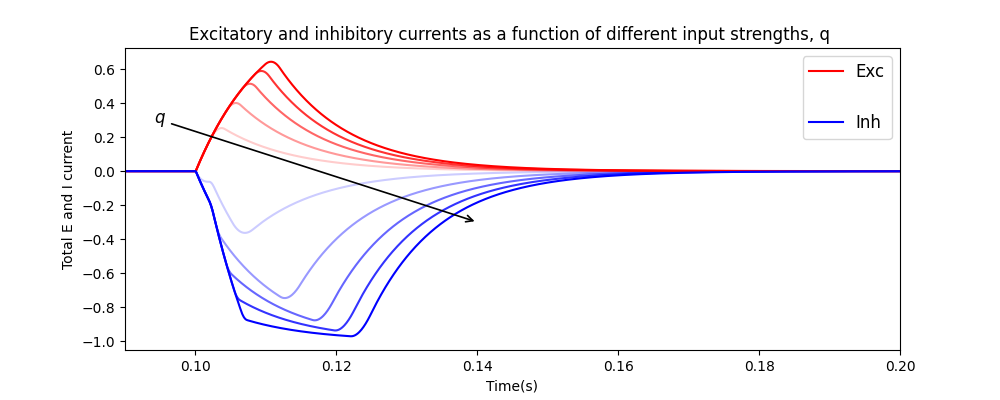
\includegraphics[width=\textwidth]{Figures/Fig9}
 \caption{ReFig9}
\end{figure}


\subsection{Reimplementation}
The iso-frequency unit model and the three-unit model were both implemented in Python and integrated into the neurolib framework \supercite{Cakan2019}.


 




\subsection{Discussion}
bla

